\documentclass[12pt]{article}

% {{{1
%%%%% preamble

%% MY PACKAGES %%%%%%%%%%%%%%%%%%%%%%%%%%%%%%%%%%%%%%%%%%%%%%%%%%%%%%%%

\usepackage{Easylayout} % \sloppy and avoid widows
\usepackage{Musthave} % must-have packages (url, unicode-math, ulem, etc.)
\usepackage{Usefancyfonts} % Gentium and Doulos (for IPA)
\usepackage{lookaheadmacros} % use "\etc," or "\etc.," to get "etc.,"
\usepackage{smallerlists} % common list environments with smaller space
%\usepackage[ % remove the author/date space.
%             % you may use \beforetitle{header text} before \maketitle
%   % sticktotop % also remove the space before the title
%]{titlecontrol}

%\usepackage{lingcontext}

%\usepackage{activechars}
%\usepackage{externalcmds}

%% POLYGLOSSIA %%%%%%%%%%%%%%%%%%%%%%%%%%%%%%%%%%%%%%%%%%%%%%%%%%%%%%%%

\usepackage{polyglossia}
%\setmainlanguage{french}
\setotherlanguage{english}
%\setotherlanguage{german}
%\setotherlanguage{greek}
%\setotherlanguage{latin}

\usepackage[
   strict,
   english=american,
   autostyle=true, % adapt for every \textLANGUAGE
   %autostyle=once, % adapt only for main language
]{csquotes}

% there is a bug: at the end of line, you may have a lonely «, and the rest of
% the sentence at the beginning of the next line; so patch:
%\DeclareQuoteStyle[patch]{french}%
%{«~}{~»}%
%{“}{”}
%\setquotestyle[patch]{french}


\MakeOuterQuote{"} %"
\MakeAutoQuote{‘}{’}


%% COMMON PACKAGES %%%%%%%%%%%%%%%%%%%%%%%%%%%%%%%%%%%%%%%%%%%%%%%%%%%%

\usepackage[
   margin=1in,
   % hmargin=2cm,
   % vmargin=2cm,
   % total={18cm,25cm}, % including header/footer, {width,height}
   % body={15cm,21cm}, % excluding header/footer, {width,height}
   includefoot, % if not set, the footer *is* in the margins
   includehead,
   % showframe
]{geometry}


%\usepackage{calc}
%\usepackage{mdframed}
%\usepackage{array}
%\usepackage{pdflscape}
%\usepackage{multirow}

%% HYPERREF %%%%%%%%%%%%%%%%%%%%%%%%%%%%%%%%%%%%%%%%%%%%%%%%%%%%%%%%%%%

\usepackage[
   bookmarks=true,
   unicode=true,
   %hidelinks=true,
   colorlinks,
   %hyperfootnotes=false
]{hyperref}

\usepackage[all]{hypcap} % references go to the top of the figure

%% SPACING %%%%%%%%%%%%%%%%%%%%%%%%%%%%%%%%%%%%%%%%%%%%%%%%%%%%%%%%%%%%

\usepackage{parskip}
%\setlength{\parskip}{8pt}
%\setlength{\parskip}{8pt plus4mm minus3mm}
\setlength{\parskip}{8pt plus4mm}
\setlength{\parindent}{0pt}

%\usepackage{setspace}
%\singlespacing
%\onehalfspacing
%\doublespacing
%\setstretch{8pt}

%% GRAPHICS %%%%%%%%%%%%%%%%%%%%%%%%%%%%%%%%%%%%%%%%%%%%%%%%%%%%%%%%%%%

%\usepackage{tikz}\usepackage{tikz-qtree}

%% EXTRA PACKAGES %%%%%%%%%%%%%%%%%%%%%%%%%%%%%%%%%%%%%%%%%%%%%%%%%%%%%

\usepackage{array}
\usepackage{mdframed}


%% COMMANDS %%%%%%%%%%%%%%%%%%%%%%%%%%%%%%%%%%%%%%%%%%%%%%%%%%%%%%%%%%%

%% EXAMPLES %%%%%%%%%%%%%%%%%%%%%%%%%%%%%%%%%%%%%%%%%%%%%%%%%%%%%%%%%%%

% {{{1
%%%%% begin document

\begin{document}

\title{SACR: User Guide}
%\beforetitle{SACR version 4.6.1\hfill Bruno Oberlé (29 mai 2017), v1.1.0}
\author{Bruno Oberle}
\date{2018-09-09\\(v0.0)}

\maketitle

\tableofcontents



%=======================                                             {{{1
 \section{Introduction}
%=======================

%~~~~~~~~~~~~~~~~~~~~~~~~~~~                                        {{{1
 \subsection{Presentation}
%~~~~~~~~~~~~~~~~~~~~~~~~~~~

SACR is an easy to use annotation tool, specifically designed to annotate
coreference chain.  It is written in HTML, CSS and Javascript, and consists in
one web page.  You can use it freely at \url{http://boberle.com/projects/sacr}
or download it from there.  It is distributed under the terms of the Mozilla
Public Licence, version 2.0 (see de \verb|LICENSE| file).

If you use it, please cite:

Oberlé B. (2018). SACR: A Drag-and-Drop Based Tool for Coreference
Annotation. \emph{Proceedings of the 11\textsuperscript{th} Edition of the
Language Resources and Evaluation Conference (LREC 2018)}. Miyazaki, Japan.

\begin{verbatim}
@inproceedings{Oberle-2018-sacr,
   author = {Bruno Oberle},
   title = "{SACR: A Drag-and-Drop Based Tool for Coreference Annotation}",
   booktitle = {Proceedings of the Eleventh International Conference on
      Language Resources and Evaluation (LREC 2018)},
   year = {2018},
   month = {May 7-12, 2018},
   address = {Miyazaki, Japan},
   editor = {Nicoletta Calzolari},
   publisher = {European Language Resources Association (ELRA)},
   isbn = {979-10-95546-00-9},
   language = {english}
}
\end{verbatim}

Remember to use Firefox (or at least Chromium or Google Chrome, but
definitevely not Internet Explorer or Edge).

With SACR, you create \emph{mentions}:

\fbox{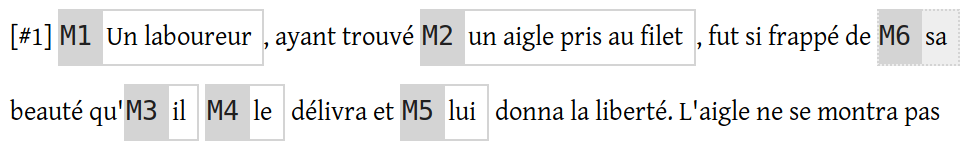
\includegraphics[width=13cm]{imgs/mentions.png}}

and you group them into \emph{sets}:

\fbox{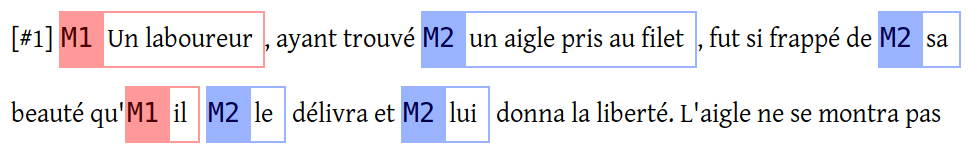
\includegraphics[width=13cm]{imgs/sets.png}}

SACR is designed to annotate coreference, so usually "mentions" are
\emph{referring expressions} and "sets" are group of referring expressions
that refers to the same referent.  These sets are sometimes called
\emph{coreference chain}.  But you can use it to annotate something else.

%~~~~~~~~~~~~~~~~~~~~~~~~~~~~~~~~~~~~                               {{{1
 \subsection{Important terminology}
%~~~~~~~~~~~~~~~~~~~~~~~~~~~~~~~~~~~~

\label{sec:terminology}

We will deal with \emph{mentions}:

\fbox{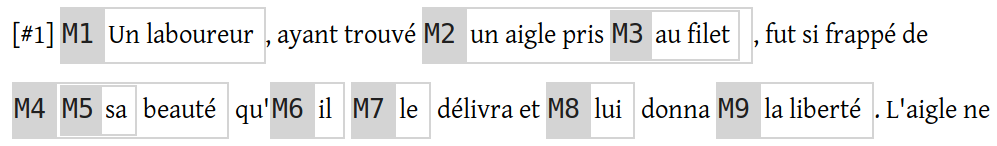
\includegraphics[width=13cm]{imgs/deal_with_mentions.png}}

Mentions can be grouped in a \emph{set} (note that the name is the same for
each member of the set):

\fbox{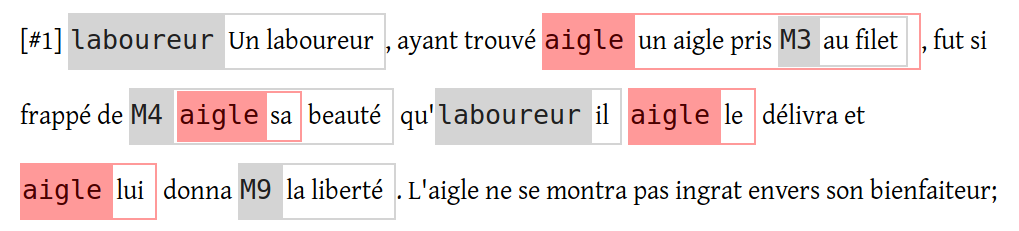
\includegraphics[width=13cm]{imgs/sets_vs_chains.png}}

When the number of mentions of a set reaches a certain threshold (usually 2
or 3, depending of the task), the are colored.  They will then be called
\emph{(coreference) chain}.  In the previous illustration, for example, the
threshold is set to 3: you see that there are five \emph{sets}: "laboureur",
"aigle", "M3", "M4", "M9", but also that there is only on \emph{chain}:
"aigle" since only this set has three elements or more.

So a \emph{mention} is an element of a \emph{set}.  A set big enough to reach
a certain threshold is called a \emph{chain}.  Note that all \emph{chains}
are \emph{set}, but that the reverse is not true.


%=====================================                              {{{1
 \section{The interface at a glance}
%=====================================

%~~~~~~~~~~~~~~~~~~~~~~~~~~                                         {{{1
 \subsection{Main window}
%~~~~~~~~~~~~~~~~~~~~~~~~~~

The figure~\ref{fig:main-interface-at-a-glance} illustrates the main
interface.  It is composed of the following elements:
\begin{enumerate}
   \item Metadata or comments in the source file.
   \item An unselected marked referring expression part of the chain
   "laboureur".
   \item A selected marked referring expression part of the chain "aigle".
   \item An unselected marked referring expression ("au filet") which isn't
   part of any chain (so it is gray).
   \item A set of features to be annotated, like the POS of the syntactic head
   of the referring expression.
   \item List of possible values for a feature.  You just have to select the
   correct one.
\end{enumerate}

\begin{figure}
\begin{center}
{%
\setlength{\fboxsep}{0pt}%
%\setlength{\fboxrule}{1pt}%
%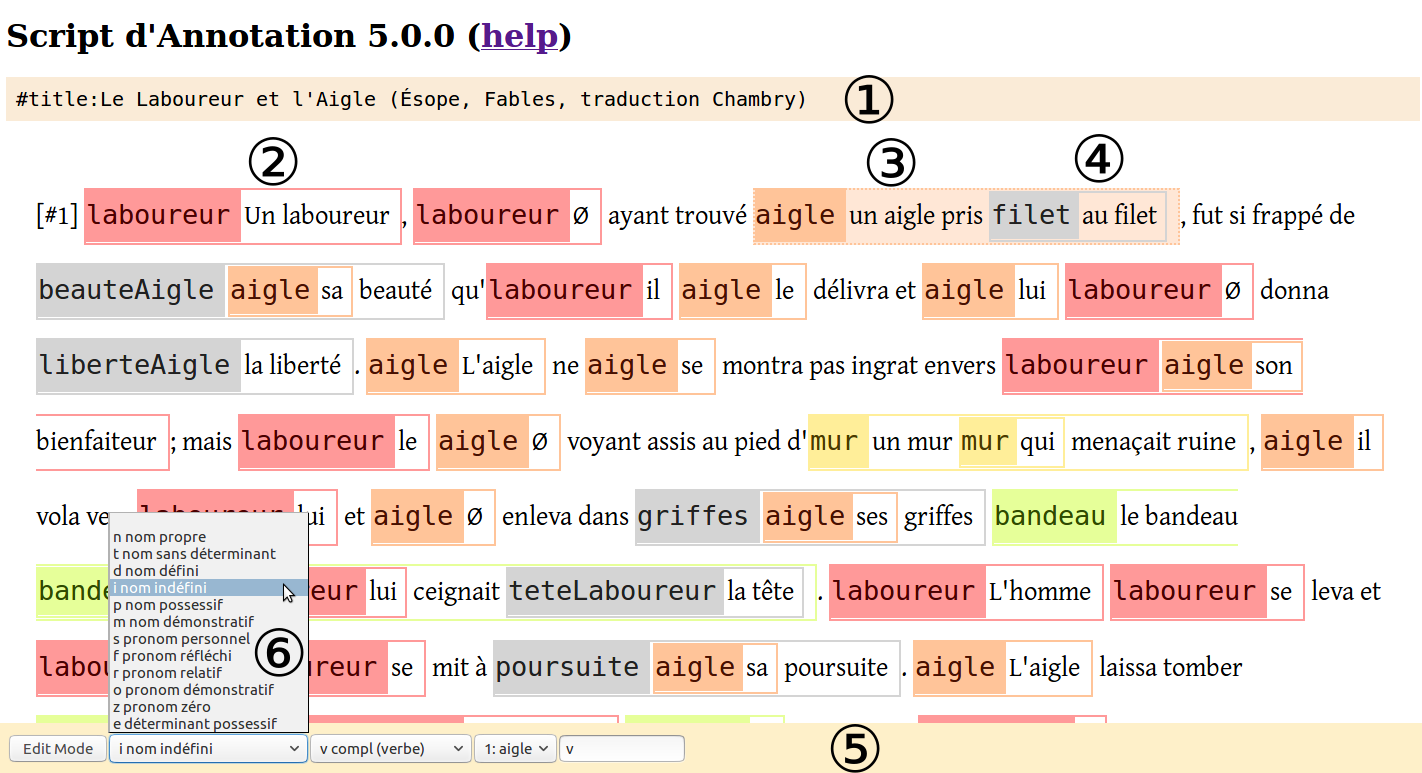
\includegraphics[width=4.8in]{imgs/main_interface_at_a_glance.png}
%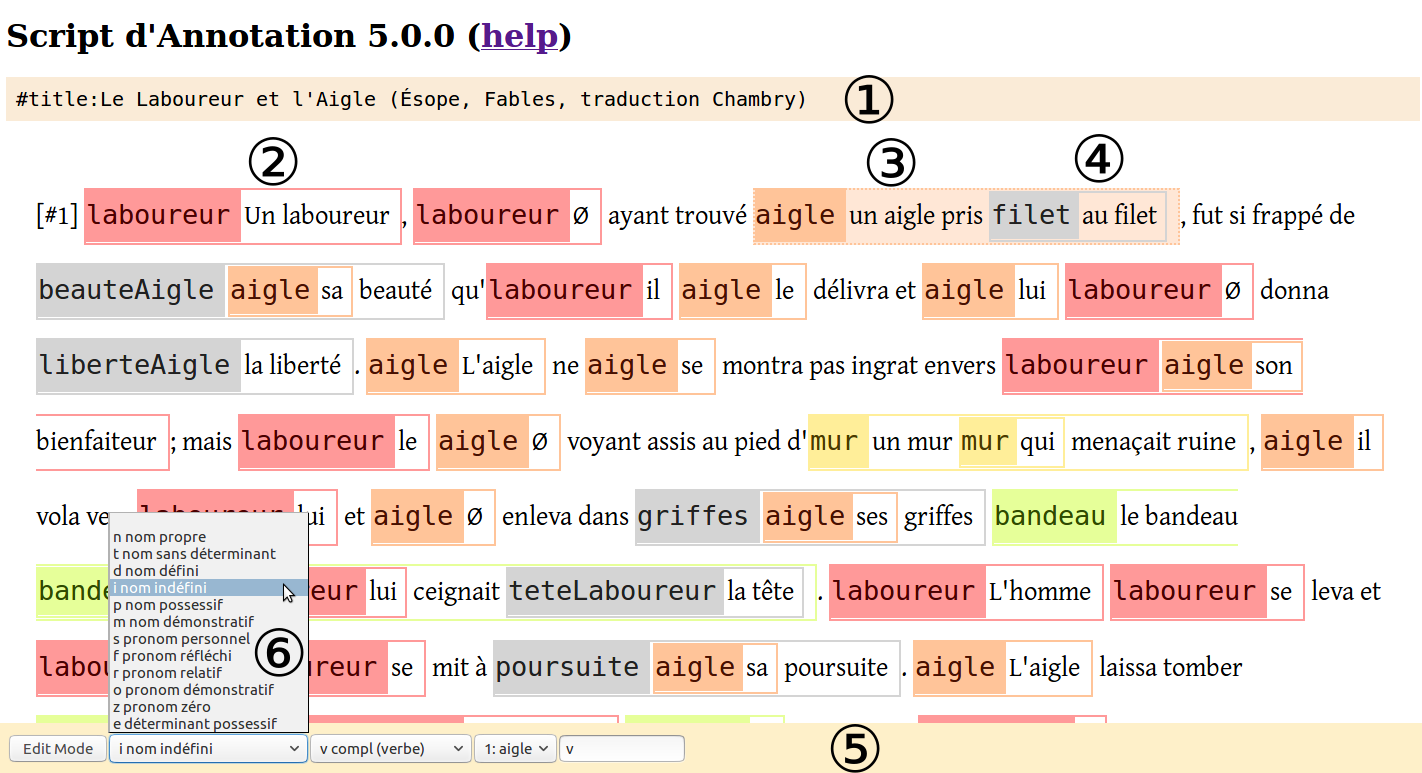
\includegraphics[scale=0.25]{imgs/main_interface_at_a_glance.png}
\fbox{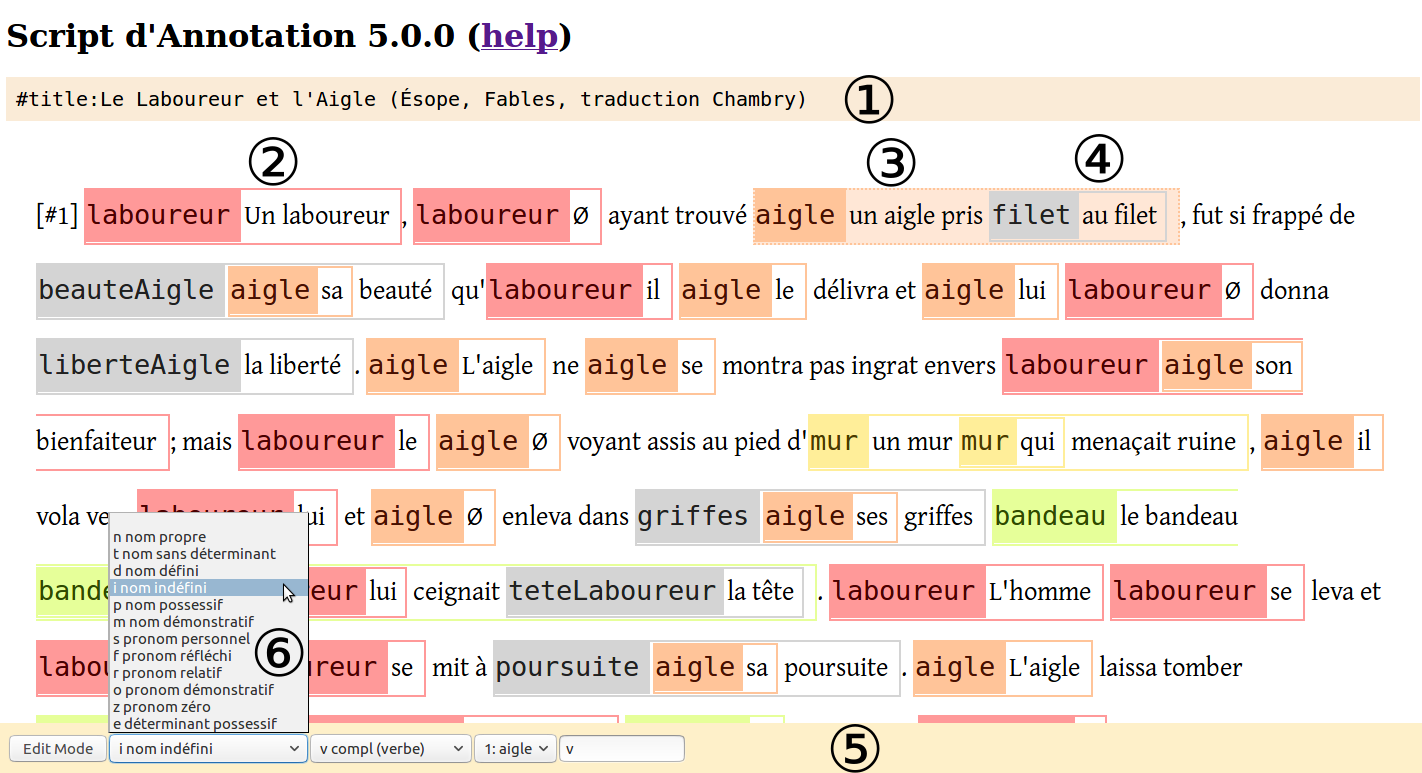
\includegraphics[width=15cm]{imgs/main_interface_at_a_glance.png}}
}
\end{center}
\caption{The main interface.}
\label{fig:main-interface-at-a-glance}
\end{figure}

As you can see, there is no control buttons.  Commands are activated by
clicking on keys on your keyboard.  For example, to change the color of a
chain, you need to press \verb|c| (as in "Color").

To get a list of all available commands, press \verb|h|.


%~~~~~~~~~~~~~~~~~~~~                                               {{{1
 \subsection{Popup}
%~~~~~~~~~~~~~~~~~~~~

The figure~\ref{fig:popup-at-a-glance} illustrates the popup window that lists
all the chains and the elements:
\begin{enumerate}
   \item The main interface in the background.
   \item The chain "laboureur" (the list of its expressions has been
   collapsed).
   \item The chain "aigle" with the list of its expressions.
   \item The expression "un aigle pris au filet" is selected both in the main
   window and in the list.  You can select in one or the other.  Note that the
   chain name "aigle" is surrounded by a black frame.
   \item Other chains with their expressions.
\end{enumerate}

\begin{figure}
\begin{center}
{%
\setlength{\fboxsep}{0pt}%
%\setlength{\fboxrule}{1pt}%
\fbox{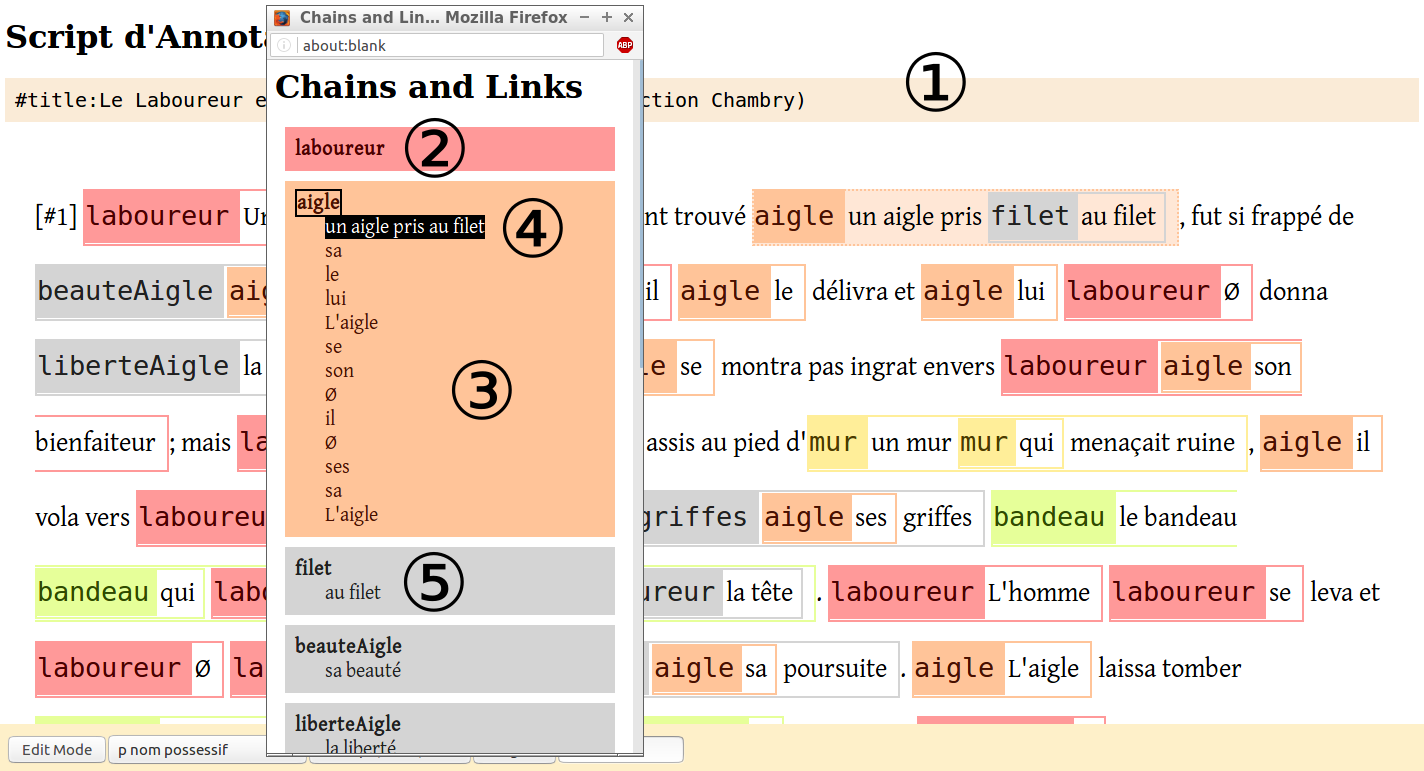
\includegraphics[width=15cm]{imgs/popup_at_a_glance.png}}
}
\end{center}
\caption{List of all chains and elements in a popup window.}
\label{fig:popup-at-a-glance}
\end{figure}

%~~~~~~~~~~~~~~~~~~~~~~~~~~~~~~~~~~~~~~~~~~~~~~~~~~~~~~             {{{1
 \subsection{What if the popup is blocked by Firefox}
%~~~~~~~~~~~~~~~~~~~~~~~~~~~~~~~~~~~~~~~~~~~~~~~~~~~~~~

Popups were often used in the 2000s to show ads.  Now they are blocked by
almost all browsers.  If, when you press \verb|p|, you get a message saying
that SACR can't create the popup, you must allow firefox to show it.

\begin{itemize}
   \item Go to the \emph{Preferences} panel of Firefox,
   \item click on \emph{Privacy \& Security}
   \item and scroll down to the \emph{Permissions} section.
\end{itemize}

For your safety, the checkbox \emph{Block pop-up windows} should be checked.

\begin{itemize}
   \item Click on the \emph{Exceptions buttons...} button,
   \item enter \verb|http://boberle.com| (and also \verb|https://boberle.com|
   for when I switch to \verb|https|),
   \item click on \emph{Allow},
   \item and click on \emph{Save changes}.
\end{itemize}

Now the \verb|p| key should show the popup.

You can follow the video at this address:
\url{http://boberle.com/projects/sacr/videos/10_allow_popup_in_firefox_exported.mp4}.
It's in French, but just follow mouse cursor, I use an English version of
Firefox.


%================================                                   {{{1
 \section{Recommended workflow}
%================================

First, create the mentions (referring expressions):\nopagebreak

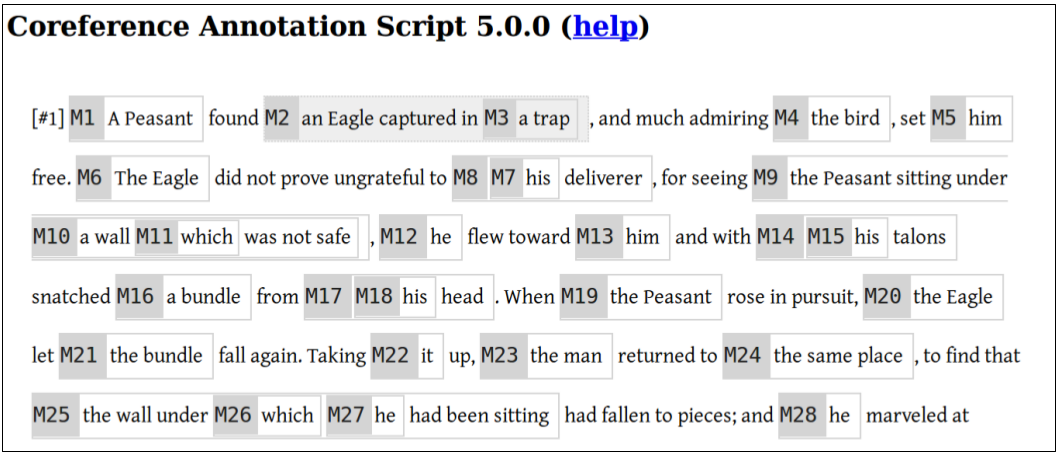
\includegraphics[width=15cm]{imgs/workflow1.png}

Second, create the sets (coreference relations):\nopagebreak

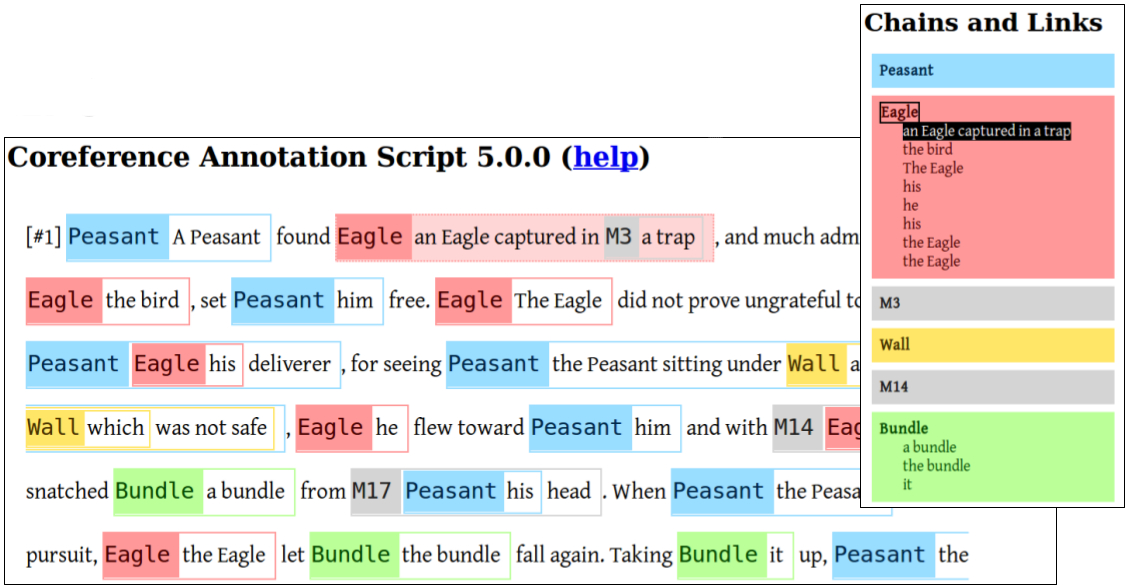
\includegraphics[width=15cm]{imgs/workflow2.png}

Third, annotated features for each mentions, if needed:\nopagebreak

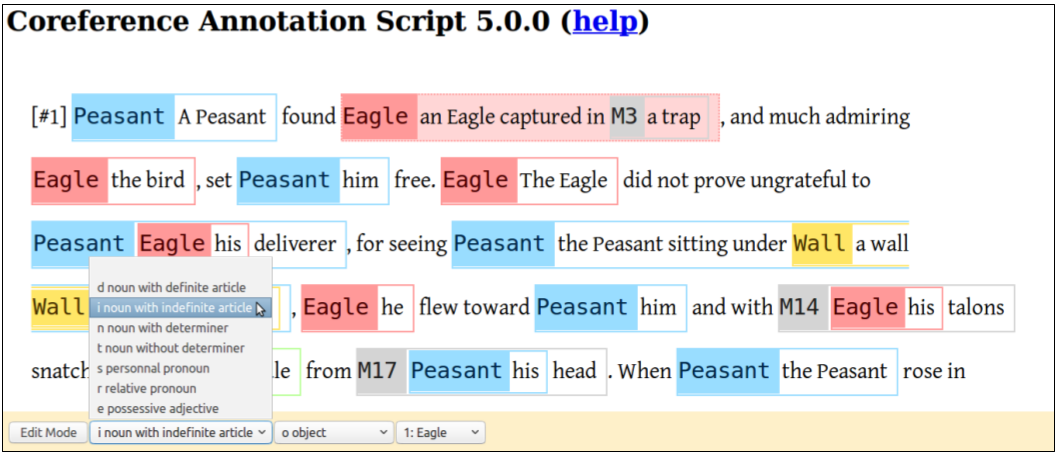
\includegraphics[width=15cm]{imgs/workflow3.png}

Fourth, visualize your data:\nopagebreak

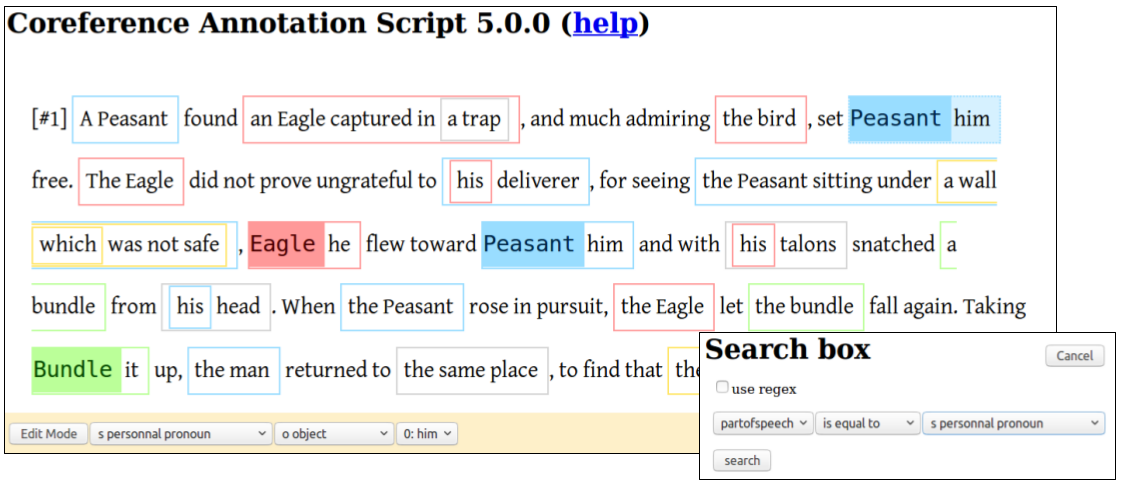
\includegraphics[width=15cm]{imgs/workflow4.png}


%=====================================================              {{{1
 \section{Creating, saving and opening a new document}
%=====================================================

%~~~~~~~~~~~~~~~~~~~~~~~~~~~~~~~~~~~~~~~~~~~                        {{{1
 \subsection{How to import or open a text with or without annotations}
%~~~~~~~~~~~~~~~~~~~~~~~~~~~~~~~~~~~~~~~~~~~

When you first open the web page, the tool will ask you to load a text and,
if you want, an annotation scheme (or schema), that is, the list of the
properties (and their possible values) you want to annotate for each
referring expression.

\begin{figure}
\begin{center}
\fbox{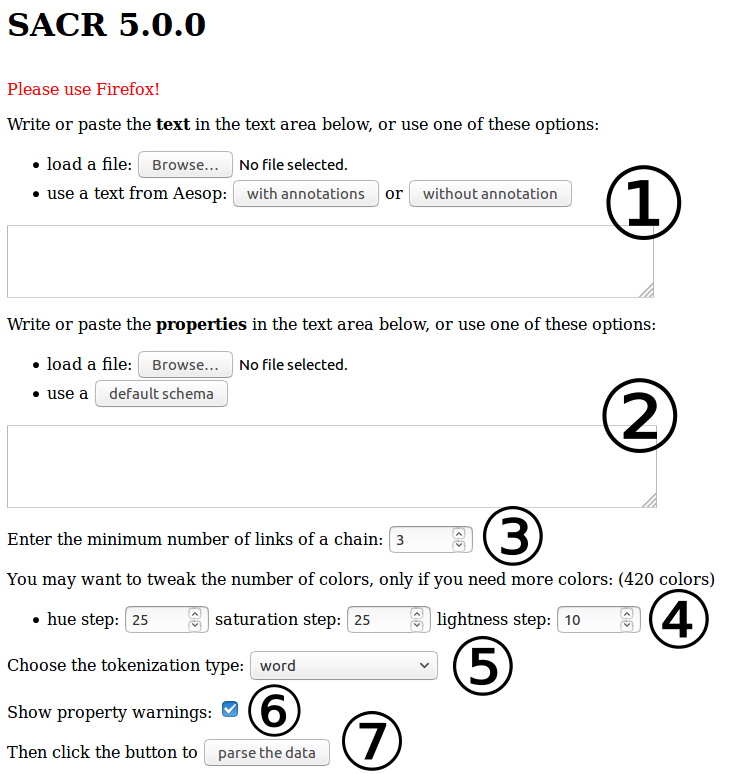
\includegraphics[width=10cm]{imgs/data_loader.png}}
\end{center}
\caption{Data loader.}
\label{fig:data-loader}
\end{figure}

To load a text with the data loader (figure~\ref{fig:data-loader}):
\begin{description}
   \item[1.] Copy a text (from the Web, Writer, Word, etc.) and copy it into the
   box, or use the button \emph{Browse} to import the text from a file stored
   on your computer.  You may also use a sample text (an Aesop's fable) with
   or without sample annotations by clicking on the buttons.
   \item[2.] If you want to annotate a set of features for each mentions, you may
   copy a schema in the next text box, or import it from a
   file stored on your computer (using the button \emph{Browse}), or use a
   default sample schema (to work with the sample texts).
   \item[3.-6.] Set up the configuration options (see
   section~\ref{sec:configuration}).
   \item[7.] Finally, just click on the \emph{parse the data} button.
\end{description}



%~~~~~~~~~~~~~~~~~~~~~~~~~~~~                                       {{{1
 \subsection{Configuration}
%~~~~~~~~~~~~~~~~~~~~~~~~~~~~

\label{sec:configuration}

See figure~\ref{fig:data-loader}.

\verb|Enter the minimum number of links of a chain|: set when a \emph{set} is
big enough to be a \emph{chain} and receive it's own color.  Usually 2 or 3,
depending of the task and the size of your text.

You may want to \verb|tweak the number of colors|, if you need more colors.
By default, there are 420 colors.  The more color you add, the less
distinctive they will be.  Play with the hue, saturation and ligthness to
increase or decrease the number of colors.

\verb|Choose the tokenization type|:
\begin{itemize}
   \item \verb|word| for normal text with latin alphabet.  Punctuation
   \emph{cannot} be selected and be a mention on their own.
   \item \verb|word| for normal text with latin alphabet.  Punctuation
   \emph{can} be selected and be a mention on their own.
   \item \verb|character|: every character can be selected individually.  Use
   this for language such as chinese or korean.
\end{itemize}

\verb|Show property warnings|: if you check this box, SACR will report an
error if there is a difference between the text and the schema you imported.
For example, if there is a property \verb|category| in the schema, but not in
the text.

%~~~~~~~~~~~~~~~~~~~~~~~~~~~~~~~~~~~~~~~~~                          {{{1
 \subsection{Text and annotation format}
%~~~~~~~~~~~~~~~~~~~~~~~~~~~~~~~~~~~~~~~~~

Annotations are inline, that means that there are stored within the text.
Metadata are also stored within the text.

The text must be in a plain text format.  Paragraph are separated by white
lines. Two consecutive non white lines are considered as been in the same
paragraph.

Here is an example:

\begin{minipage}{\linewidth}
\begin{mdframed}
\begin{verbatim}
This is a sentence
of the first paragraph...
which continues here...
and even here!

After the white line, this starts the
second paragraph.
\end{verbatim}
\end{mdframed}
\end{minipage}

Metadata are added as lines that start with \verb|#|.  Some metadata are used
by SACR itself, as \verb|#COLOR|.  While \verb|#textid| and \verb|#title| are
not mandatory, they are exploited by SACR to display the text id and the
title in the browser window title bar.  Other metadata may be used to
organize the corpus (as \verb|#textid|, \verb|#title|, \verb|#source|, etc.)
or by the tool that performs the statistical analysis (for example, to
distinguish between parts (introduction, body, conclusion, etc.):

\begin{mdframed}
\begin{verbatim}
#textid: 1
#title: text title
This is the text...
\end{verbatim}
\end{mdframed}

Two metadata are important:
\begin{itemize}
   \item Lines starting with \verb+#additionnaltoken:new token+ are used to
   define additionnal tokens.  For example if you want a symbol (like "α") to
   be recognized as chunk of text that you can annotate, you can use this
   metadata.
   \item Lines starting with \verb+#part-heading:level=1+ indicate that the
   following paragraph is a heading.  This is used for a better layout.
\end{itemize}

Annotations are stored as follows:

\verb+{ReferentName:prop1="val1",prop2="val2" text inside the mention}+

For example:

\begin{mdframed}
\begin{verbatim}
{chat:categorie="SN défini",fonction="sujet" Le petit chat de
{voisine:categorie="SN défini",fonction="cdn" la voisine}}
\end{verbatim}
\end{mdframed}

See figure~\ref{fig-sacr-example-text} for a complete example.

\begin{figure}[tbp]
\begin{mdframed}
\begin{verbatim}
#title:Le Laboureur et l'Aigle (Ésope, Fables, traduction Chambry)

{laboureur:categorie="i nom indéfini",fonction="s sujet",head="1:
laboureur",expansion="" Un laboureur}, {laboureur:categorie="z pronom
zéro",fonction="s sujet",head="0: Ø",expansion="" Ø} ayant trouvé
(...)

************************************************************************

Il faut rendre (...)

#COLOR:green=laboureur
#COLOR:blue=aigle
#COLOR:orange=mur
#COLOR:red=bandeau
#DEFAULTCOLOR:gray
\end{verbatim}
\end{mdframed}
\caption{Text example.}\label{fig-sacr-example-text}
\end{figure}


%~~~~~~~~~~~~~~~~~~~~~~~~~~~~~~~~~~~~~~~~~~~~~~~~~~~~~~~~~~~~       {{{1
 \subsection{Saving the annotations and opening them later}
%~~~~~~~~~~~~~~~~~~~~~~~~~~~~~~~~~~~~~~~~~~~~~~~~~~~~~~~~~~~~

Before leaving the page, you need to save your annotations in a file.  Just
press \verb|w| (as in "Write").  Depending on your browser settings, the file
will be saved automatically (usually in your "Downloads" directory) or you
will be asked where to store it.

The filename will include a time stamp (that is, the current date and time).
This allows you to save several versions of the same file.

Imagine you have loaded a file called \verb|esope|.  When you press the
\verb|w| key, SACR will save a file called \verb|esope_20170529_230130|
(where \verb|20170529_230130| is the date (year, month, day) and time (hours,
minutes, seconds).

If you save the some minutes later, you get, for example,
\verb|esope_20170529_230424| (the name ends with \verb|0424| instead of
\verb|0130|).

If you copied a text in the text area without using the \emph{browse} button
on the data loader, you get a name like \verb|default_20170529_230130|.

The next annotation session, you just load (using the "browse" button of the
data loader) the last file you saved, for example
\verb|esope_20170529_230424| or \verb|default_20170529_230130|.

%============================================                       {{{1
 \section{Creating and editing annotations}
%============================================

%~~~~~~~~~~~~~~~~~~~~~~~~~~~~~~~~                                   {{{1
 \subsection{Creating mentions}
%~~~~~~~~~~~~~~~~~~~~~~~~~~~~~~~~

\label{sec:creating-mentions}

To create singletons:
\begin{itemize}
   \item if the mention have only one word: double click on that word,
   \item if the mention has several words:
     \begin{itemize}
         \item click on the first word (it is then underlined; to cancel and
         choose another word, just click again on it and it will be
         un-underlined),
         \item click on the last word.
      \end{itemize}
\end{itemize}

Batch mode:
\begin{itemize}
   \item select a mention,
   \item create mention as before, but hold \verb|ctrl|: all the newly
   created mentions will be automatically attached to the mention you
   selected in the first step.
\end{itemize}

Example of the batch mode:
\begin{itemize}
   \item Let's say you have the sentences: "Paul est heureux.  Il est
   content. Il est joyeux."
   \item Create a mention for "Paul" and then select it.
   \item Hold \verb|ctrl| and double-click on the first "il" and the second
   "il".
   \item Both "il" are attached to "Paul": you have create the set "Paul...
   Il... Il..." with a minimal effort!
\end{itemize}



%~~~~~~~~~~~~~~~~~~~~~~~~~~~~~~~~~~~~~~~~~~~~~~~~~~~~               {{{1
 \subsection{Creating sets (coreference relations)}
%~~~~~~~~~~~~~~~~~~~~~~~~~~~~~~~~~~~~~~~~~~~~~~~~~~~~

Let's say you have several mentions, and you want to group them (for example
because they are coreferential).

%-------------------------------------                              {{{1
 \subsubsection{Using drag-and-drop}
%-------------------------------------

You just need to drag-and-drop one mention one over another.  The mention
that is attached to the set will get the name of the set.  If the set reach
the critical size to be chain (see the terminology in
section~\ref{sec:terminology}), then it will be colored.

There are some behavior differences depending of the source and the
destination, but the process is designed to be intuitive.  Here is the
detail (note that a "singleton" is a set with one element, and a "group", in
the table, a set with more than one element):

\begin{tabular}{c|c|m{10.5cm}}
\textbf{source} & \textbf{destination}& \textbf{result}\\\hline
singleton & singleton& destination is attached to the source\\\hline
singleton & group & source is attached to the destination (1)\\\hline
group & singleton & destination is attached to the source\\\hline
group & group & groups are merged (SACR will ask you to confirm) (2)\\
\end{tabular}

Notes:
\begin{itemize}
   \item (1) If you want to detach the destination from its group and
   attached to the source, hold \verb|ctrl|.
   \item (2) If you don't want to merge, but just detach the destination from
   its group and attached it to the source, hold \verb|ctrl|.
\end{itemize}

It's a bit abstract, but in fact it's intuitive.  Just practice!


%---------------------------------------------------                {{{1
 \subsubsection{Example 1: singleton to singleton}
%---------------------------------------------------

Drag the singleton \emph{Un laboureur} and drop it over the singleton
\emph{il}:\nopagebreak

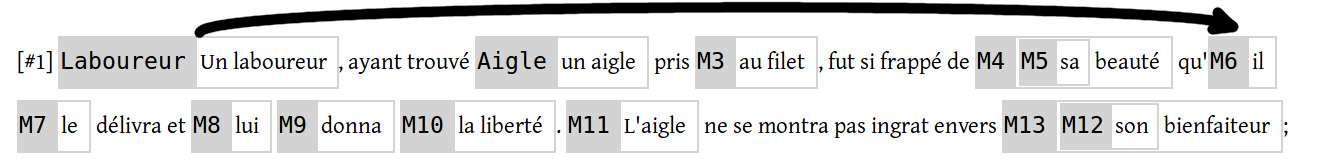
\includegraphics[width=17cm]{imgs/dd_example_01_before.png}

The mention \emph{il} is attached to \emph{Un laboureur}:\nopagebreak

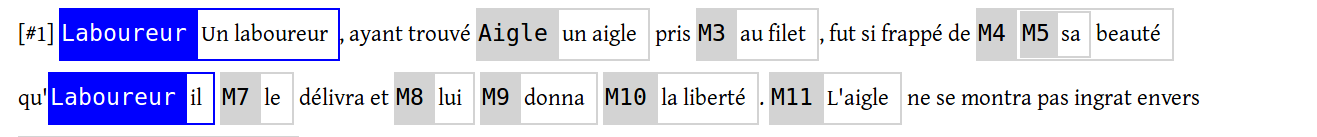
\includegraphics[width=17cm]{imgs/dd_example_01_after.png}


%-----------------------------------------------                    {{{1
 \subsubsection{Example 2: singleton to group}
%-----------------------------------------------

Drag the singleton \emph{donna} and drop it over one of the mentions of the
group, here for example \emph{Un laboureur}:\nopagebreak

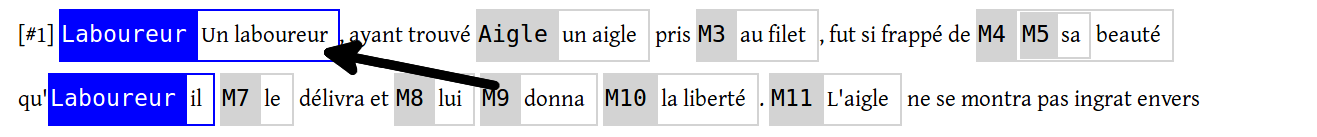
\includegraphics[width=17cm]{imgs/dd_example_02_before2.png}

The mention \emph{donna} is attached to the group:\nopagebreak

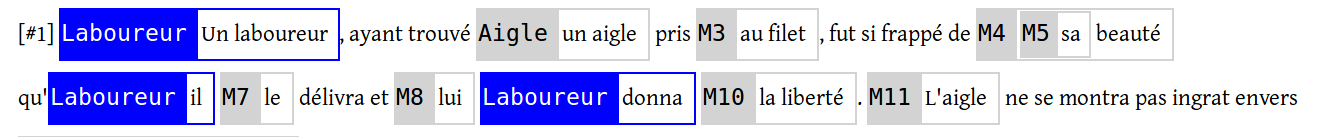
\includegraphics[width=17cm]{imgs/dd_example_02_after.png}

%-----------------------------------------------                    {{{1
 \subsubsection{Example 3: group to singleton}
%-----------------------------------------------

Do the opposite: drag one of the mentions of the group, here for example
\emph{Un laboureur} and drop it over the singleton \emph{donna}:\nopagebreak

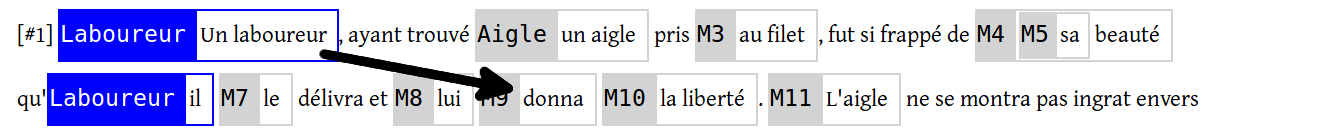
\includegraphics[width=17cm]{imgs/dd_example_02_before.png}

You get the same result as before:\nopagebreak

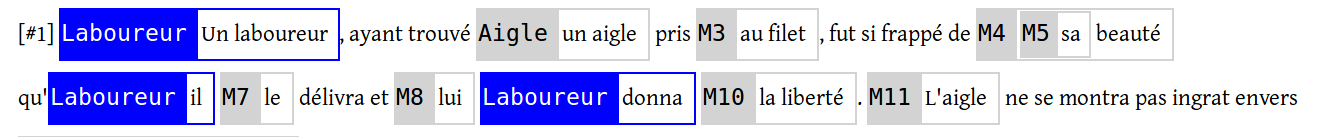
\includegraphics[width=17cm]{imgs/dd_example_02_after.png}

%-------------------------------------------                        {{{1
 \subsubsection{Example 4: group to group}
%-------------------------------------------

\label{sec:merging-example}

Drag one of the mentions of a group, here for example \emph{Un laboureur},
and drop it over one of the mentions of another group, here for example 
\emph{lui}:\nopagebreak

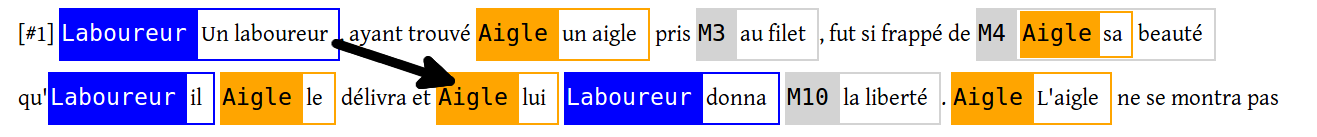
\includegraphics[width=17cm]{imgs/dd_example_03_before.png}

You will be ask if you want to merge:\nopagebreak

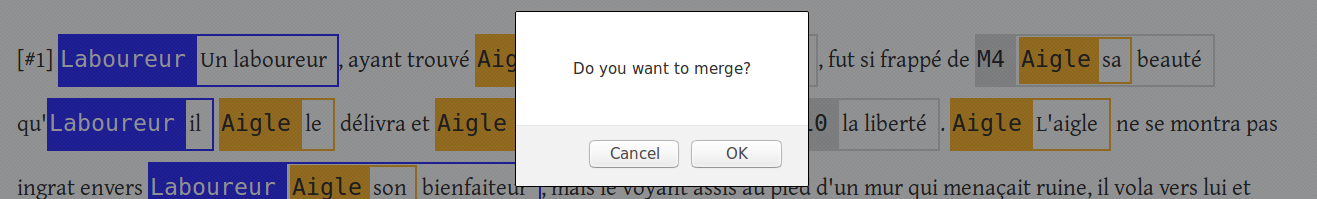
\includegraphics[width=17cm]{imgs/dd_example_03_dialog.png}

If yes:\nopagebreak

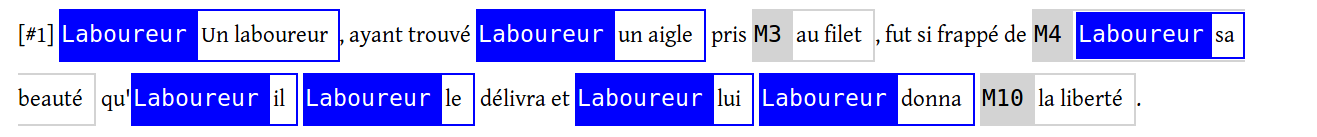
\includegraphics[width=17cm]{imgs/dd_example_03_after.png}

%------------------------------------------------                   {{{1
 \subsubsection{Example 5: Using \texttt{ctrl}}
%------------------------------------------------

If you hold \verb|ctrl|, you detach the destination mention (here \emph{un
aigle}) from its group:\nopagebreak

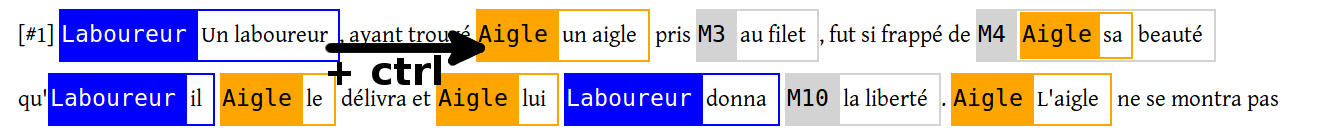
\includegraphics[width=17cm]{imgs/dd_example_04_before.png}

to attach it to the source group:\nopagebreak

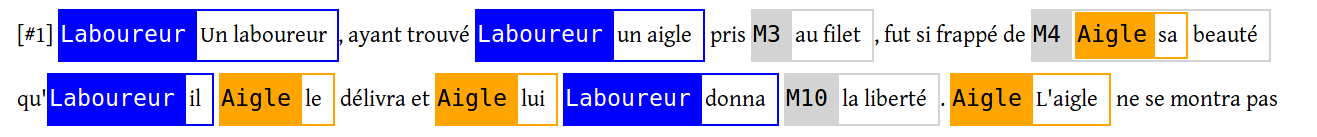
\includegraphics[width=17cm]{imgs/dd_example_04_after.png}

%--------------------------------------------------                 {{{1
 \subsubsection{Using \texttt{ctrl} (batch mode)}
%--------------------------------------------------

\begin{itemize}
   \item Select a mention,
   \item hold \verb|ctrl| and click on other mentions: they will all be
   attached to the mention you selected in the first step.
\end{itemize}

Example of the batch mode:
\begin{itemize}
   \item Let's say you have the sentences: "Paul est heureux.  Il est
   content. Il est joyeux."
   \item Create a mention for "Paul", "Il" and "Il".
   \item Select "Paul".
   \item Hold \verb|ctrl| and click on the other two mentions.
   \item Now, they all belong to the same group!
\end{itemize}

You can use this if you have a to relate to distant mentions.  Select the
first, scroll down to the second one and click on it.

%~~~~~~~~~~~~~~~~~~~~~~~~~~~~~~~~~~                                 {{{1
 \subsection{Selecting a mention}
%~~~~~~~~~~~~~~~~~~~~~~~~~~~~~~~~~~

Don't confuse "selecting (or clicking on) a mention" and "selecting (or
clicking on) a word".  You select a word by clicking on it: it is underlined.
You do that to create a new mention (you need to click on another word to
complete the process, see section~\ref{sec:creating-mentions}).  If you have
selected a word by error, just click on it a second time to deselect it.

To "select (or click on) a mention", you need to click on its name (the part
with the colored background) or anywhere on the white part inside the frame
of the mention, except on a word (in which case you select a word...).  To
deselect a mention, click on it.

See figure~\ref{fig:select-expr} for some examples.

When you select a word, all mentions are deselected, and vice-versa.

\begin{figure}
\begin{mdframed}
\begin{itemize}
   \item The \textbf{word} \emph{sa} is selected (since it is underlined):\par
   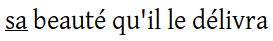
\includegraphics[scale=0.5]{imgs/sa_selected.png}
   \item The \textbf{mention} \emph{un aigle} is selected:\par
   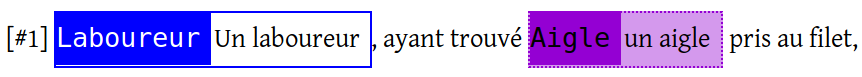
\includegraphics[scale=0.5]{imgs/aigle_selected.png}
   \item The \textbf{mention} \emph{un laboureur} is selected:\par
   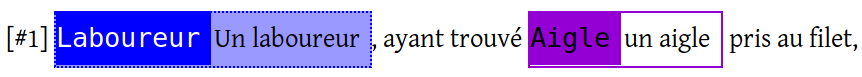
\includegraphics[scale=0.5]{imgs/laboureur_selected.png}
   \item The \textbf{mention} \emph{qui} is selected.  It is nested in
   another mention:\par
   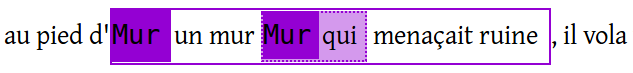
\includegraphics[scale=0.5]{imgs/qui_selected.png}
   \item The \textbf{mention} \emph{un mur qui menaçait ruine} is selected.
   Another mention is nested (\emph{qui}), which is not selected.  Look at
   the dashed frame around \emph{un mur qui menaçait ruine} (selected), and
   the solid frame around \emph{qui} (not selected):\par
   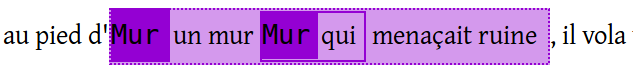
\includegraphics[scale=0.5]{imgs/un_mur_selected.png}
   \item To select a \textbf{mention}, click on the name (with the colored
   background) (black arrow), or anywhere in the white area (red arrow).  The
   first method is easier:\par
   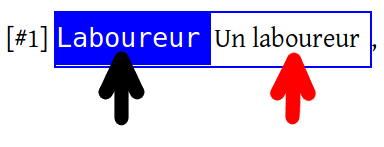
\includegraphics[scale=0.5]{imgs/select_refex.png}
\end{itemize}
\end{mdframed}
\caption{Word and mention selectin.}\label{fig:select-expr}
\end{figure}

%~~~~~~~~~~~~~~~~~~~~~~~~~~~~~~~~~~~~~~~~~~~~~                      {{{1
 \subsection{Detaching an element from a group}
%~~~~~~~~~~~~~~~~~~~~~~~~~~~~~~~~~~~~~~~~~~~~~

Hold \verb|shift| and click on the mention you want to detach: it will be
grayed and renamed with a name as \verb|M123| (using the next available
counter value).  It is now a singleton.

%~~~~~~~~~~~~~~~~~~~~~~~~~~~~~~~                                    {{{1
 \subsection{Merging two sets}
%~~~~~~~~~~~~~~~~~~~~~~~~~~~~~~~

Drag-and-drop the element of one set over the element of another set.  You
will be ask if you really want to merge.

The name of the resulting set is the name of the name of the source.

See example in section~\ref{sec:merging-example}.

%~~~~~~~~~~~~~~~~~~~~~~~~~~~~~                                      {{{1
 \subsection{(Re)naming a set}
%~~~~~~~~~~~~~~~~~~~~~~~~~~~~~

Select a mention of the set and and press:
\begin{itemize}
   \item \verb|N| to change the name of the selected chain (don't ask,
   use the content of the selected mention),
   \item \verb|n| to change the name of the selected chain (ask,
   default is current name),
   \item \verb|m| to change the name of the selected chain (ask,
   default is the content of the selected mention).
\end{itemize}

%~~~~~~~~~~~~~~~~~~~~~~~~~~~~~~~~~~~~~~~~~~                         {{{1
 \subsection{Changing the color of a chain}
%~~~~~~~~~~~~~~~~~~~~~~~~~~~~~~~~~~~~~~~~~~

Reminder: a set has a color only only if it is a chain, that is if it is has
as many elements as indicated in the
\verb|Enter the minimum number of links of a chain| textbox (see
section~\ref{sec:configuration}).  Other sets (not chains) are in gray.

Select a mention of the chain and press \verb|c|.  Choose the color and click
on "cancel" (top-right corner).


%=====================================                              {{{1
 \section{Searching and visualizing}
%=====================================

%~~~~~~~~~~~~~~~~~~~~~~~~~~~~~~~~~~~                                {{{1
 \subsection{Displaying only one set}
%~~~~~~~~~~~~~~~~~~~~~~~~~~~~~~~~~~~

Select a mention of the set and press \verb|o|.  Press \verb|O| to show all
mentions.

Press \verb|u| to hide all sets that are not chains.

%=====================                                              {{{1
 \section{The popup}
%=====================

TODO


%======================================================================{{{1
 \section{Command reference and all other commands that aren't listed
 elsewhere in this guide}
%======================================================================

Type \emph{h} to show the main available commands (see figure~\ref{fig:help}).

\begin{figure}[tbp]
\begin{center}
\fbox{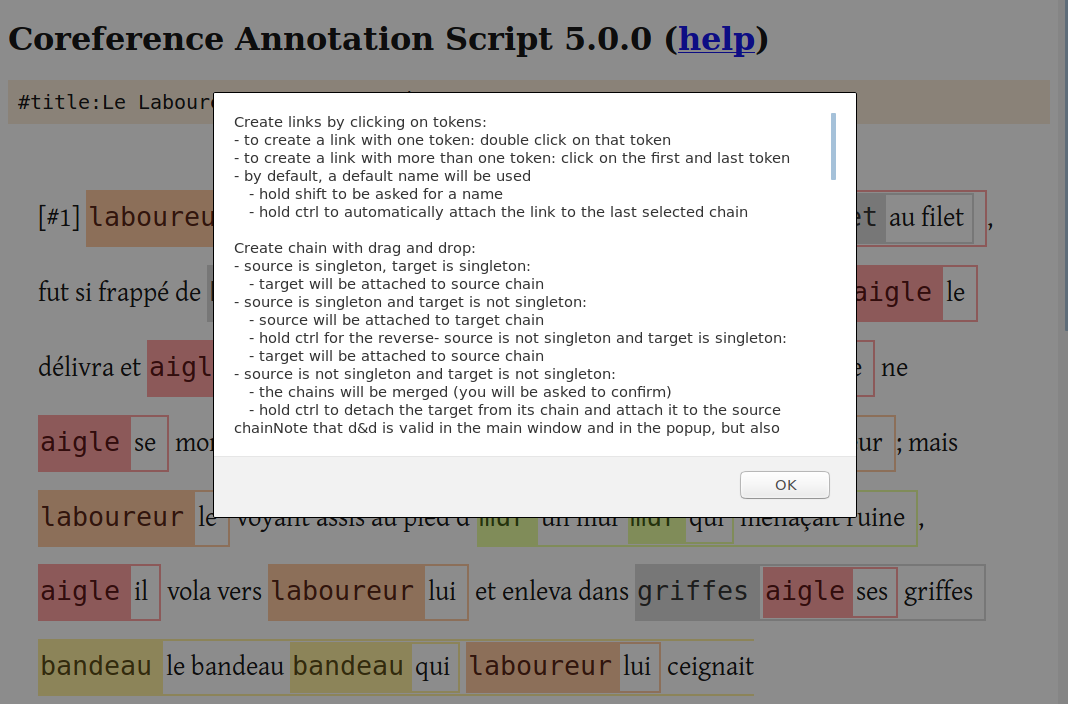
\includegraphics[width=15cm]{imgs/help.png}}
\end{center}
\caption{Help!}
\label{fig:help}
\end{figure}

\paragraph{Creating mentions}  To create a mention, click on the first and
the last word of the mention.  If the mention has only one word, just
double click on it.  A default name will be used, or:
\begin{itemize}
   \item hold \verb|shift| to be asked for a name,
   \item hold \verb|ctrl| to automatically attach the link to the last
      selected set.
\end{itemize}

\paragraph{Creating coreference relation} To attach a mention to an other (to
create a "coreference relation"), drag-and-drop one mention over another.

Severals cases are possible (see below for illustrations):
\begin{itemize}
   \item source is singleton, target is singleton:
      \begin{itemize}
      \item target will be attached to source chain,
      \end{itemize}
   \item source is singleton and target is not singleton:
      \begin{itemize}
      \item source will be attached to target chain
      \item hold \verb|ctrl| for the reverse
      \end{itemize}
   \item source is not singleton and target is singleton:
      \begin{itemize}
      \item target will be attached to source chain
      \end{itemize}
   \item source is not singleton and target is not singleton:
      \begin{itemize}
      \item the chains will be merged (you will be asked to confirm)
      \item hold \verb|ctrl| to detach the target from its chain and attach
      it to the source chain
      \end{itemize}
\end{itemize}

Note that d\&d is valid in the main window and in the popup, but also between
them.

\paragraph{Replacing a mention} To replace a mention, create a new mention,
then drag-and-drop, holding \verb|shift| (or \verb|ctrl+shift| for Firefox 54
and below), it to the mention to be replaced.  This will copy all the metadata
(mention name and properties) to the target mention, and remove the source
mention.

\paragraph{Detaching a mention from its set} To detach the mention, you
can either:
\begin{itemize}
   \item hold \verb|shift| and click on a mention.  The mention will be a
   singleton and its name will change to something like \verb|M123| (next
   available counter value),
   \item hold \verb|ctrl+shift| and click on a mention.  The mention will be
   a singleton but you will be ask a name (rather than \verb|M123|),
   \item hold \verb|ctrl| and click on a mention.  The mention will be
   attached to a the last selected set.
\end{itemize}

\paragraph{Editing links} Use:
\begin{itemize}
   \item \verb|suppr| or \verb|backspace| to destroy the selected mention,
   \item \verb|c| to change the color of the selected set,
   \item \verb|N| to change the name of the selected set (don't ask, use
   the content of the selected mention),
   \item \verb|n| to change the name of the selected set (ask, default is
   current name),
   \item \verb|m| to change the name of the selected set (ask, default is
   the content of the selected mention).
\end{itemize}

\paragraph{Navigating} Use:
\begin{itemize}
   \item \verb|f| to go forward in text,
   \item \verb|F| to go forward in text (only visible),
   \item \verb|j| to go forward in set,
   \item \verb|J| to go forward in set (only visible),
   \item \verb|b| to go backward in text,
   \item \verb|B| to go backward in text (only visible),
   \item \verb|k| to go backward in set,
   \item \verb|K| to go backward in set (only visible),
   \item \verb|t| to scroll to the selected mention in the main window,
   \item \verb|T| to scroll to the selected mention in the popup window.
\end{itemize}

\paragraph{Showing and hiding mentions} Use:
\begin{itemize}
   \item \verb|o| to show only the set of the selected mention,
   \item \verb|O| to show all mentions,
   \item \verb|s| to show the search box,
   \item \verb|u| to hide non chains,
   \item \verb|U| to hide/show (toggle) non chains in popup,
\end{itemize}

\paragraph{Popup} Use:
\begin{itemize}
   \item \verb|p| to show the popup window of all sets and mentions,
   \item \verb|e| to expand all sets in the popup,
   \item \verb|E| to collapse all sets in the popup,
   \item \verb|v| to expand chains in the popup.
\end{itemize}

\paragraph{Saving} Use:
\begin{itemize}
   \item \verb|w| to write the text and annotations to a file,
   \item \verb|W| to write the text and annotations to a file (with head text
   and link content),
   \item \verb|x| to write the schema to a file,
   \item \verb|X| to show the schema (in a dialog).
\end{itemize}

\paragraph{Displaying}
\begin{itemize}
   \item \verb|i| to increase font size,
   \item \verb|I| to decrease font size,
   \item \verb|l| to whow statistics,
   \item \verb|P| to show chain patterns.
\end{itemize}


%======================================                             {{{1
 \section{Setting mention properties}
%======================================

%~~~~~~~~~~~~~~~~~~~~~~~~~~~~                                       {{{1
 \subsection{Schema format}
%~~~~~~~~~~~~~~~~~~~~~~~~~~~~

A schema is a list of all the properties you want to annotate for mentions,
and all the their possible values.  You don't need a schema if you just want
to annotate coreference.  But a schema is required if you want to annotate
the part the speech, the grammatical function, etc. for each mention.

See figure~\ref{fig-sacr-example-schema} for an example which describes the
main options.

\begin{figure}[tbp]
\begin{mdframed}
\begin{verbatim}
# line beginning with # are comments (i.e. there are ignored

# a new property beginning with PROP: and a serie of parameters
PROP:name=partofspeech
# the following line means "blank", no value
$$$
proper name
indefinite noun phrase
definite noun phrase
...

# properties are separated by a white line

PROP:name=fonction
$$$
subjet
object
...

# a property of type "text" allows users to put anything they want
PROP:name=comment,type=text

# the head property is special, see below
PROP:name=head,type=head
\end{verbatim}
\end{mdframed}
\caption{Sample schema.}\label{fig-sacr-example-schema}
\end{figure}

You may add other parameters (in the form \verb|param1=val1,param2,val2|
etc.):
\begin{itemize}
   \item \verb+newline=true|false+: add a new line characters after the
   property (use that if you have lot of properties),
   \item \verb+showname=true|false+: show the name of the property, not just
   a text box or a list of values,
   \item \verb+textboxsize=4+: if type is \verb|text|, set the size of the
   textbox (4 for example),
   \item \verb+addShortcuts=true|false+: automatically add shortcut keys for
   the quick mode (see section~\ref{sec:quick-mode}).
\end{itemize}

%~~~~~~~~~~~~~~~~~~~~~~~~~~~~~~~~~~~~~~~~~~~~~~~~~~~~~~~~~~~        {{{1
 \subsection{How to change the schema after the annotation is started}
%~~~~~~~~~~~~~~~~~~~~~~~~~~~~~~~~~~~~~~~~~~~~~~~~~~~~~~~~~~~

If you want to change the schema after the annotation is started, you must
load the annotations and the new schema as usual, but be careful \emph{not}
to check the \verb|Show property warnings| checkbox.

SACR will automatically remove the properties that don't appear in the new
schema, add the properties that don't appear in the current annotation state,
and adapt the values.  Of course, you will need to manually annotated the new
properties and check the values if needed.



%~~~~~~~~~~~~~~~~~~~~~~~~                                           {{{1
 \subsection{Slow mode}
%~~~~~~~~~~~~~~~~~~~~~~~~

TODO

%~~~~~~~~~~~~~~~~~~~~~~~~~                                          {{{1
 \subsection{Quick mode}
%~~~~~~~~~~~~~~~~~~~~~~~~~

\label{sec:quick-mode}

TODO

%================                                                   {{{1
 \section{Misc}
%================

%~~~~~~~~~~~~~~~~~~~~~~~~~~~~~~~~~~~~~~~~~~~~~~~~~~~~~~~~~~         {{{1
 \subsection{How to convert from and to the Glozz format}
%~~~~~~~~~~~~~~~~~~~~~~~~~~~~~~~~~~~~~~~~~~~~~~~~~~~~~~~~~~

TODO


% {{{1
%%%%% end document

\end{document}


